\section{Examples Illustrating the Previous Chapters (6K)}

% -- Chart 1 -----------------------------------------------42-
An example: \Sun\xspace in \Cancer\xspace 29° 30', \Moon\xspace in \Pisces\xspace 12°, \Saturn\xspace in \Sagittarius\xspace 27° 8', \Jupiter\xspace in \Capricorn\xspace 22° 13' <7°?>, \Mars\xspace in \Scorpio\xspace 7° 23', \Venus\xspace in \Cancer\xspace 28° 13', \Mercury\xspace in \Leo\xspace 11° 25',
Ascendant in \Pisces\xspace 17°, MC in \Sagittarius\xspace 25°
\footnote{\textit{Greek Horoscopes} dates the chart (L75) to approximately July 19, 75 AD (p.87)}. 

\clearpage
\begin{wrapfigure}[15]{R}{7cm}
\centering
\vspace{-20pt}
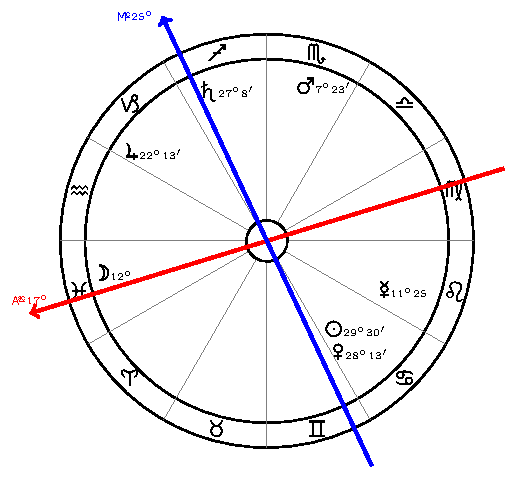
\includegraphics[width=0.68\textwidth]{charts/3_06_1}
\caption{Chart 42 [III.06.1, GH L75]}
\label{fig:chart42}
\end{wrapfigure} 

\noindent The nativity was without a houseruler because \Venus,
the ruler of \textbf{/142K/} the terms of the \Moon, had already set. The apheta was the Ascendant. 

\noindent \Mercury, the ruler of its <Ascendant’s> terms, was itself found just preceding the Descendant. Thus the vital sector
extends from the Ascendant to the point square <\Gemini\xspace 17°>, and to the projection of rays on the part of \Saturn\xspace into the point in opposition <to \Saturn: \Gemini 27°> to \Saturn, which is in the terms of a malefic <\Saturn>. \Mars\xspace deflected its diametrically opposite ray because \Jupiter\xspace was found in an equivalent degree and hindered the anaeretic influence. 

The native died at age 69, but if \Jupiter\xspace trine had not hindered <this malign influence>, he would have lived only 64 years.
\newpage
% -- Chart 2 ----------------------------------------------43-
Another example: \Sun\xspace in \Pisces\xspace 25° 8', \Moon\xspace in \Gemini\xspace 16° 53', \Saturn\xspace in \Pisces\xspace 1° 25', \Jupiter\xspace in
\Sagittarius\xspace 24° 18', \Mars\xspace in \Taurus\xspace 21° 8', \Venus\xspace in \Aquarius\xspace 9°, \Mercury\xspace in <\Aries 12°>, Ascendant in \Libra\xspace 15°, MC at \Cancer\xspace 16°
\footnote{\textit{Greek Horoscopes} dates the chart (L110) to approximately March 15, 110 AD (p.105)}.  

\clearpage
\begin{wrapfigure}[15]{R}{7cm}
\centering
\vspace{-20pt}
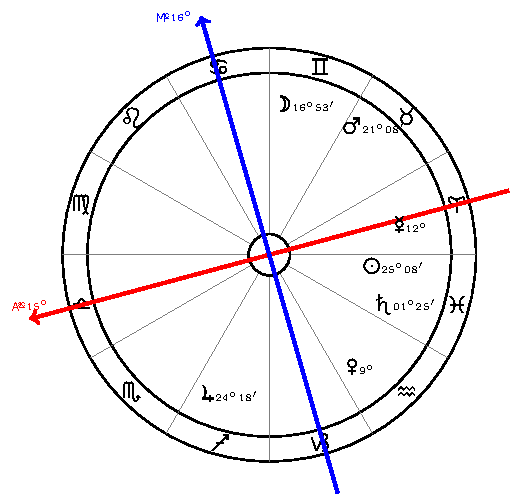
\includegraphics[width=0.68\textwidth]{charts/3_06_2}
\caption{Chart 43 [III.06.2, GH L110]}
\label{fig:chart43}
\end{wrapfigure} 

The luminaries preceded the angles <MC Descendant>, the Ascendant was the apheta in the terms of \Jupiter, and \Jupiter\xspace was unfavorably situated\footnote{Because he was declining in the 3rd, not within the vital sector and in \Saturn's terms and square to him?}. The nativity lacked a houseruler, and the vital sector was <from the Ascendant> to \Scorpio\xspace 21°, the point in opposition to \Mars. \Mars, located in the aphetic terms <of \Jupiter> and casting rays into the same terms, was the anaereta. The
native died in his 51st year.

The aphetic\mn{Aphetic \& Anaeretic Terms} terms and the anaeretic terms (i.e. the terms of malefics) are not only those degrees in which the destructive stars are found or into which they cast their rays, but also those where the vital sector
is in the beginning of the term <of a malefic>. In addition, it is necessary to calculate not only the chronocratorship of the sign which receives the ray, but also that of the sign which casts the ray, the sign in which the anaereta is found.

\ldots
\newpage